\section{Le plateau de Jeu}

\subsection{Représentation du plateau}
\label{sec:plateau_de_jeu}
Le plateau de jeu est représenté par un graphe dont les noeuds sont exactement les cases du palier. Pour manipuler le graphe, la bibliothéque GSL (GNU Scientific Library) est utilisée. C'est une bibliothéque numérique pour les programmeurs C et C ++ qui fournit dans le cadre de ce projet des fonctions qui manipulent des matrices creuses. Ce qui permet de modéliser le graphe en considérant une matrice d'adjacence t de taille $n\times n $ qui vérifie la propriété t[i][j] = 1 si et seulement s'il existe une arrête entre le noeud i et le noeud j où n est le nombre de sommet du graphe. Une autre matrice o est définie de taille $2\times n$ qui vérifie que o[k][i] = 1 si et seulement si le noeud i est occupé par le joueur k.
Plus précisément, une structure nommé \textbf{graph\_t} représente le graphe. Elle est constituée du nombre total de noeud et des deux matrices creuses citées précédemment:
\begin{lstlisting}[language={C},captionpos=b, frame=single]
    struct graph_t {
  size_t num_vertices;  // Number of vertices in the 
  gsl_spmatrix* t;  
  gsl_spmatrix* o;      
};
\end{lstlisting}
Dans ce projet, nous travaillons avec trois types de graphe de taille variable à savoir le graphe hexagonal, carré et triangulaire représentés sur la figure suivante.
\begin{figure}[h]
    \centering
    \label{fig:Hexgraph}
    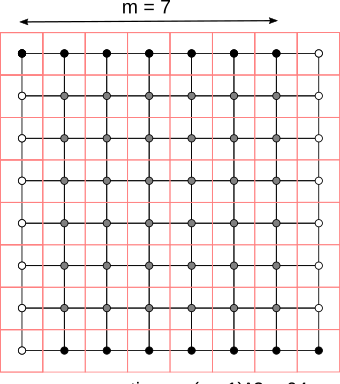
\includegraphics[width=0.3\textwidth]{Images/carre.png}
    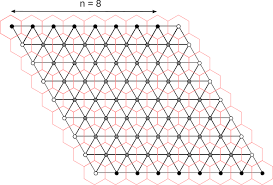
\includegraphics[width=0.5\textwidth]{Images/hexagonal.png}
    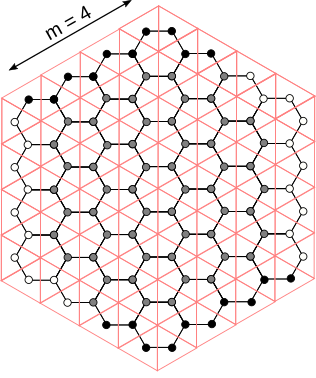
\includegraphics[width=0.3\textwidth]{Images/triangulaire.png}
    \caption{Les types de graphe utilisés}
\end{figure}

\subsection{Les coups de jeu}

Nous représentons un coup de jeu par une structure \textbf{struct move\_t} qui contient le numéro du noeud choisi par le joueur ainsi que la couleur du joueur. 
\begin{lstlisting}[language={C},captionpos=b, frame=single]
    struct move_t {
    size_t m; 
    enum color_t c;
\end{lstlisting}

On choisi les couleurs: BLACK = 0 et WHITE = 1 pour désigner les joueurs. Le joueur de couleur Noir est celui qui commence la partie de jeu.  

\subsection{Les coups de jeu}
